\section{Allgm. Wissen}
\subsection{Analog}
	\begin{compactitem}
		\item Die reale Welt ist analog (z.B. Sinnesorgane)
		\item Die analoge Verarbeitung stellt das Ergebnis einer Berechnung praktisch sofort zur Verfügung.
		\item Analoge Systeme sind anfällig auf externe Störsignale.
		\item Analoge Systeme sind extrem aufwändig und erfordern viel Fachwissen.	
	\end{compactitem}
	
\subsection{Digital}
	\begin{compactitem}
		\item Einfacher automatisierbarer Entwurf und Test mit Hilfe von CAD möglich.
		\item Digitale Schaltungen werden als integrierte Schaltungen mit Transistoren hergestellt uns sind somit reproduzierbar.
		\item Digitale Systeme sind bis zu einem gewissen Grad weitgehend immun gegen Störsignale.
	\end{compactitem}
	
\subsection{Unterschied Analog zu Digital}
\begin{multicols}{3}
	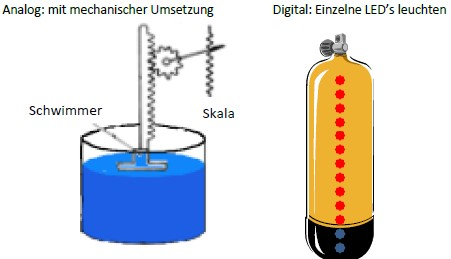
\includegraphics[width=5cm]{pics/unterschied_analog_digital.jpg}
		\columnbreak
	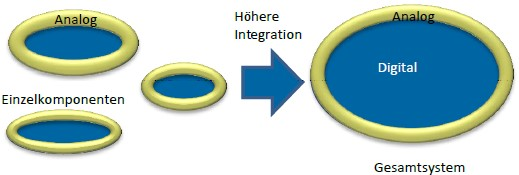
\includegraphics[width=5cm]{pics/analog_digital_integration.jpg}
		\columnbreak
		\\
	Trend zu höherer Integration: Der digitale Anteil wächst, wobei der analoge Teil weiterhin die Verbindung nach Aussen darstellt \lbrack wie eine Schale\rbrack.
\end{multicols}

	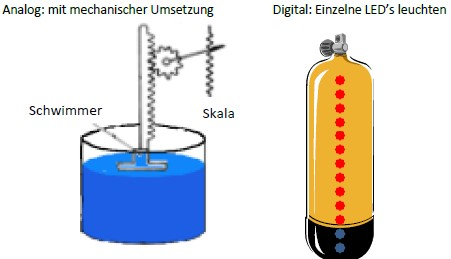
\includegraphics[width=0.3\textwidth]{pics/unterschied_analog_digital.jpg}
	
	\subsubsection{Integration}
		\begin{minipage}[c]{8 cm}
			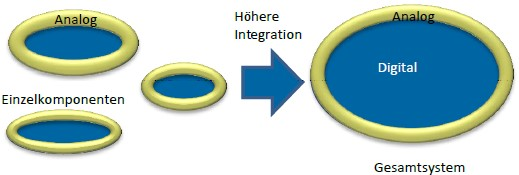
\includegraphics[width=0.9\textwidth]{pics/analog_digital_integration.jpg}
		\end{minipage}
		\begin{minipage}[c]{10 cm}
			Trend zu höherer Integration: Der digitale Anteil wächst, wobei der analoge Teil weiterhin die Verbindung nach Aussen darstellt \lbrack wie eine Schale\rbrack.
		\end{minipage}
	
\subsection{Codes}
	\begin{minipage}[c]{5 cm}
		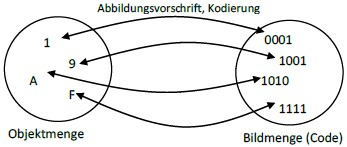
\includegraphics[width=0.9\textwidth]{pics/codes.jpg}
	\end{minipage}
	\begin{minipage}[c]{13 cm}
		Folgende Codes werden am häufigsten gebraucht:
		\begin{compactitem}
			\item Binärcode
			\item 
				\begin{tabbing}
					xxxxxxxxxxxxxxx\=xxxxxxxxxxxxxxxxxxxxxxxxxxxxxxxx\kill	
					Reiner Dualcode: \> Zuordnung von Dezimalzahlen den Bitfolgen des Dualsystems
				\end{tabbing}
			\item 
				\begin{tabbing}
					xxxxxxxxxxxxxxx\=xxxxxxxxxxxxxxxxxxxxxxxxxxxxxxxx\kill
					BCD Code: \> 
								\begin{tabular}{|lllllll|}
									\hline
										Dezimal & 1 & 2 & 3 & $\dots$ & 9 & \textgreater 9 \\
										BCD & 0001 & 0010 & 0011 & $\dots$ & 1001 & ungültig\\
									\hline
								\end{tabular}
				\end{tabbing}
		\end{compactitem}
	\end{minipage}

\subsection{Begriffe im Zusammenhang mit dem binären Zahlensystem}
	\begin{compactitem}	
		\item 
			\begin{tabbing}
				xxxxxxxxxxx\=xxxxxxxxxxxxxxxxxxxxxxxxxxxxxxxxxxxxx\kill	
				Bit (b): \>
							Binary Digit: Kleinsmögliche Speichereinheit in der Digitaltechnik. Kann zwei mögliche Zustände\\
				 		\>	annehmen: 0 und 1
			\end{tabbing}
		\item 
			\begin{tabbing}
				xxxxxxxxxxx\=xxxxxxxxxxxxxxxxxxxxxxxxxxxxxxxxxxxxx\kill	
				Byte (B): \>
							Einheit von 8 Bits. Auch genannt Oktett: 1 Oktett = 1 Byte = 8 Bit. Byte ist die Standartbezeichnung\\
						\>	von Speicherkapazitäten und Datenmengen.
			\end{tabbing}
		\item 
			\begin{tabbing}
				xxxxxxxxxxx\=xxxxxxxxxxxxxxxxxxxxxxxxxxxxxxxxxxxxx\kill	
				Nibble: \>
							Binärzahlen in Gruppen von 4 Bits
			\end{tabbing}
		\item 
			\begin{tabbing}
				xxxxxxxxxxx\=xxxxxxxxxxxxxxxxxxxxxxxxxxxxxxxxxxxxx\kill	
				MSB: \>
							Most Significant Bit. Bit mit höchster Wertigkeit, steht ganz links im binären Wort
			\end{tabbing}
		\item 
			\begin{tabbing}
				xxxxxxxxxxx\=xxxxxxxxxxxxxxxxxxxxxxxxxxxxxxxxxxxxx\kill	
				LSB: \>
							Least Significant Bit. Bit mit tiefster Wertigkeit, steht ganz rechts im binären Wort
			\end{tabbing}
	\end{compactitem}

	\begin{minipage}{8 cm}
	Weil sequentielle Schaltungen in der Regel synchron arbeiten, muss eine Referenz zur Einhaltung der Synchronit"at definiert werden. Das Taktsignal ist ein bin"ares Signal, das in regelm"assiger Abfolge zwischen zwei Zust"anden hin und her pendelt.
	\end{minipage}a

	\subsubsection{Unterschied Flipflop und Latch}
		\begin{minipage}{12 cm}
			Taktzustandsgesteuerte Systeme haben den Nachteil, dass in ihrer transparenten Phase auch asynchrone Schaltvorg"ange stattfinden k"onnen. Echt synchrone Systeme "andern ihren Zustand nur bei der aktiven Flanke des Taktsignals. Genau in diesem Moment und sonst nie wird das Eingangssignal bei einem Speicherelement in den Speicher "ubertragen. Nur beim taktflankengesteuerten System wechseln die Ausg"ange immer genau zum Zeitpunkt der aktiven Taktflanke. Beim taktzustandsgesteuerten System sind w"ahrend der transparenten Phase auch Zustands"anderungen zwischen zwei Taktflanken m"oglich. \\
			Taktflankengesteuerte Speicherelemente werden Flip-Flops genannt. Taktzustandsgesteuerte Speicherelemente werden Latches genannt
		\end{minipage}
		\begin{minipage}{0.5 cm}
			\ 
		\end{minipage}
		\begin{minipage}{6 cm}
			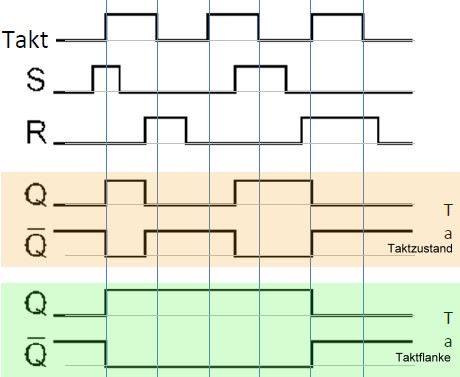
\includegraphics[width=0.9\textwidth]{pics/flipflop_latch}
		\end{minipage}